\section{Acquisition vidéo}

\subsection{Cadence et réglage du grain de l'image}

L'horloge pixel est ce qui permet de définir la cadence de balayage du capteur, c'est donc la période qui sépare deux
balayages de la matrice de pixels. Cette horloge pixel a des valeurs bornées avec un minimum de 8 MHz et
un maximum de 40MHz. Après avoir fait varier cette valeur, nous avons vu que l'horloge n'avait pas d'impact
direct sur l'image. En revanche, l'horloge pixel a un impact sur d'autres paramètres de l'image. Elle plafonne les valeurs
de la cadence d'acquisition et du temps d'intégration.\newline

On peut voir que lorsqu'on augmente la cadence d'acquisition et que le temps d'intégration est très bas, l'image
clignote quand la pièce est éclairée avec de la lumière artificielle. Ce phénomène est dû à un décalage de phase entre
la caméra et le courant alternatif alimentant la lumière.\newline

Le temps d'intégration est le temps durant lequel le capteur reçoit les photons permettant de constituer l'image.
Lorsque ce temps est trop bas, on remarque que la luminosité de l'image baisse également. En effet, plus ce
temps est bas, moins le capteur reçoit d'énergie et l'image s'assombrit. À l'inverse, plus cette période est longue,
plus le nombre de photons reçus par le capteur est grand et plus l'image est lumineuse. Cependant, cela peut entrainer un effet de bougé,
car si l'objet bouge, le capteur va récupérer de l'énergie de ses différentes positions.\newline

\begin{figure}[H]
      \center
      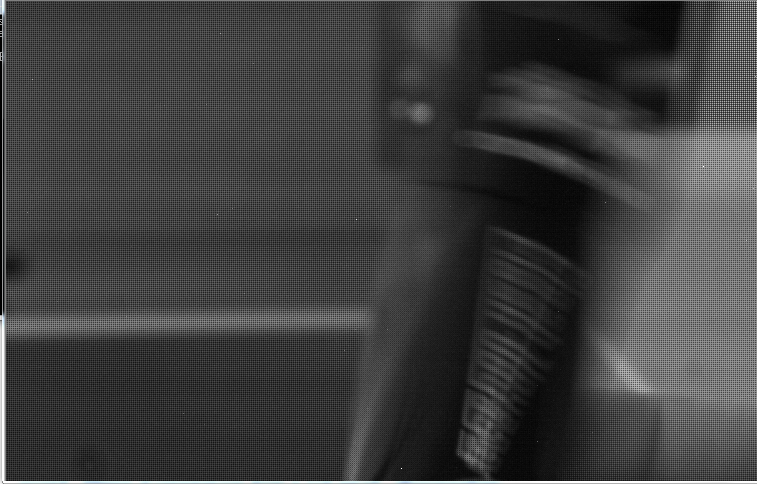
\includegraphics[width=10cm]{ressources/tp2/flou_de_bouge.PNG}
      \caption{Illustration du flou de bougé}
\end{figure}

Le gain est une sorte d'amplificateur du signal. Plus le gain est grand, plus l'image sera lumineuse.
En revanche si le gain est trop grand, l'image va perdre de sa qualité et risque de contenir du grain. En effet, le gain amplifie également le bruit du signal, ce qui donne ce grain très caractéristique.\newline

\subsection{Taille de l'image}

A partir du code fourni, on peut voir qu'il est possible de récupérer certaines informations concernant la caméra.
On peut, par exemple, récupérer la résolution maximale du capteur de la caméra qui est de 752x400.\newline

Lorsque l'on réduit la taille de la zone d'intérêt, on voit que l'image qui est récupérée correspond au coin supérieur
gauche de l'image. Cependant, c'est le coin inférieur droit du capteur qui est balayé par l'électronique de la caméra 
et qui reçoit la lumière de la zone d'intérêt.\newline

On voit que lorsque l'on divise la taille de l'image, il est possible de déplacer celle-ci dans l'ensemble de la zone 
délimitée par la définition maximale du capteur. On peut donc arriver au calcul suivant : 
\begin{framed}
$$ iPosx + iSizeX <= iMaxSizeX$$
$$ iPosx <= iMaxSizeX - iSizeX$$
\end{framed}

Le binning est le fait de regrouper des pixels en utilisant l'ensemble de la surface du capteur. Ceci a pour conséquence
de réduire l'image que l'on voit sur l'ordinateur. Si on modifie le binning X, l'image se réduit horizontalement et 
si on modifie le binning Y, l'image se réduit verticalement.\newline

%question 5 pas oK

\subsection{Images N et B et couleur}

Pour obtenir une image en noir et blanc (i.e. en niveaux de gris) à partir d'une image couleur, il n'est pas nécessaire de modifier le nombre de bits, ni
le nombre de canaux car les niveaux de gris sont codés sur 8 bits et n'ont besoin que d'un seul canal. A l'inverse, pour passer d'une image couleur à une image en niveaux de gris,
il faut passer à trois canaux (rouge, vert, bleu) et modifier le nombre de bits à 24, 8 bits pour chaque canal.\\

Avec un arrangement des pixels de type Bayer, et en regroupant les pixels par 2 à la verticale, on obtient une image qui ne tient plus compte des nuances de vert car les pixels correspondant
ont été regroupés avec les autres du fait de l'alternance des pixels verts et des autres.

\begin{figure}[H]
      \center
      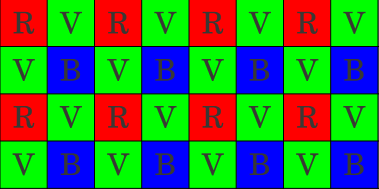
\includegraphics[width=8cm]{ressources/tp2/Bayer.png}
      \caption{Arrangement de type Bayer}
\end{figure}

Nous remarquons que si nous mettons le même gain sur chaque couleur, l'image paraît plus verte. En effet, l'homme est 
capable de voir plus de variantes de la couleur verte que des autres couleurs et le capteur de la caméra comporte plus 
de pixels associés à la couleur verte. C'est pourquoi il faut ajuster les gains
de chaque couleur pour observer une image qui paraît bien proportionnée au niveau des couleurs.\\

%revoir le binning

%si gain egale -> il y aura plus de vert
%binning -> desactive pixel vert à cause du regroupement

%voir si cette partie est bien terminé
